\documentclass[11pt,letterpaper]{article}
\usepackage[T1]{fontenc}
\usepackage{mathptmx}
\usepackage[scaled=0.90]{helvet}
\usepackage{microtype}
\usepackage[margin=1in]{geometry}
\usepackage{amsmath,amssymb,amsthm}
\usepackage{booktabs}
\usepackage{array}
\usepackage{tikz}
\usetikzlibrary{arrows.meta,positioning,calc}
\usepackage{enumitem}
\usepackage{titlesec}
\usepackage{fancyhdr}
\usepackage{framed}
\usepackage{xcolor}
\usepackage[colorlinks=true,linkcolor=black,urlcolor=black,citecolor=black]{hyperref}

\definecolor{shadecolor}{gray}{0.93}
\setcounter{tocdepth}{2}

\pagestyle{fancy}
\fancyhf{}
\lhead{\small ECON 601 \textbullet{} Lecture 1: Preferences}
\rhead{\small\thepage}
\renewcommand{\headrulewidth}{0.4pt}

\theoremstyle{definition}
\newtheorem{defn}{Definition}
\newtheorem{axiom}{Axiom}
\theoremstyle{plain}
\newtheorem{thm}{Theorem}
\newtheorem{prop}{Proposition}
\newtheorem{lem}{Lemma}

\newcommand{\src}[1]{{\small\textsf{(#1)}}}
\newcommand{\fwd}[1]{\textsf{\textbf{$\rightarrow$ #1:}}}
\newcommand{\bwd}[1]{\textsf{\textbf{$\leftarrow$ #1:}}}
\newcommand{\wpref}{\succsim}
\newcommand{\spref}{\succ}
\newcommand{\indif}{\sim}
\newcommand{\Rn}{\mathbb{R}^n_+}
\newcommand{\MRS}{\mathrm{MRS}}
\newcommand{\MU}{\mathrm{MU}}
\newcommand{\skipnote}{\noindent{\small\textsf{Proof. Skippable on a first read.}}\par\smallskip}

\setlist{itemsep=1pt,topsep=3pt}

\title{\vspace{-2.2em}\textbf{Lecture 1: Preferences}\\[0.3em]
\large ECON 601, with the ideas before the formulas}
\author{}
\date{}

\begin{document}
\maketitle
\vspace{-3em}
\begin{center}
\small \textbf{How to read this.} Each section opens with a concrete situation and a plain-English
claim. The formal statement follows. Proofs sit in ruled blocks and can be skipped entirely on a
first pass; nothing later depends on having read them. One consumer with real numbers runs through
the whole document.\\[0.4em]
Sources: Lectures 1--3 (L1--L3), Review Sessions 1--2 (RS1--RS2), Problem Set 1 (PS1),
Jehle \& Reny 3rd ed.\ (J\&R).
\end{center}
\vspace{0.8em}

{\small\tableofcontents}
\vspace{1em}

\section{Why any of this exists}

\subsection{The problem: tastes are invisible}

Suppose you want to predict what someone buys when the price of coffee changes. To do that with
calculus you need a function to maximize. So you need a number attached to every possible basket of
goods, and that number has to come from somewhere.

The nineteenth-century answer was that pleasure is a measurable substance and utility is how much of
it you get \src{J\&R p.4}. Nobody can check that. You cannot open a person and read off how many
units of satisfaction a sandwich delivers.

Modern theory starts from far less. The only thing assumed observable is that a person, shown two
baskets, can say which one she likes at least as well. That is all. Lecture 1 is the machine that
turns that single ability into a number a computer can maximize, and it is scrupulous about
recording how much of that number is real and how much is bookkeeping.

Lecture 2 then maximizes the number subject to a budget. Lecture 3 studies the maximized value.
Everything downstream consumes the output of this lecture, which is why the assumptions made here
determine what is provable there.

\begin{center}
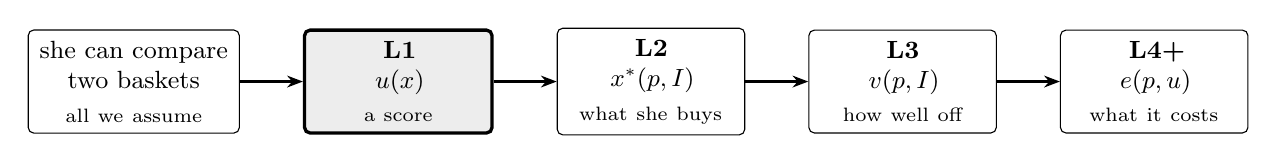
\begin{tikzpicture}[
  node distance=8mm,
  box/.style={draw,rounded corners=2pt,align=center,inner sep=4pt,font=\small,minimum height=12mm,text width=21mm},
  focus/.style={box,very thick,fill=shadecolor},
  arr/.style={-{Stealth[length=2mm]},thick}
]
\node[box,text width=24mm] (prim) {she can compare\\two baskets\\[1pt]{\scriptsize all we assume}};
\node[focus,right=of prim] (l1) {\textbf{L1}\\$u(x)$\\[1pt]{\scriptsize a score}};
\node[box,right=of l1] (l2) {\textbf{L2}\\$x^*(p,I)$\\[1pt]{\scriptsize what she buys}};
\node[box,right=of l2] (l3) {\textbf{L3}\\$v(p,I)$\\[1pt]{\scriptsize how well off}};
\node[box,right=of l3] (l4) {\textbf{L4+}\\$e(p,u)$\\[1pt]{\scriptsize what it costs}};
\draw[arr] (prim) -- (l1);
\draw[arr] (l1) -- (l2);
\draw[arr] (l2) -- (l3);
\draw[arr] (l3) -- (l4);
\end{tikzpicture}
\end{center}

\subsection{Mei, for the rest of the document}

Every claim below is illustrated on one person. Mei is choosing weekly baskets of coffees and
lunches. Her tastes happen to be Cobb-Douglas with equal weight, $u = \sqrt{x_1 x_2}$, though for
most of this document we will not assume that and will only use three of her rankings.

\begin{center}
\begin{tabular}{@{}llcc@{}}
\toprule
\textbf{Basket} & \textbf{Contents} & \textbf{Her score} & \textbf{Score under a different labelling} \\
\midrule
A & 16 coffees, 4 lunches & 8 & 64 \\
C & 8 coffees, 8 lunches & 8 & 64 \\
B & 4 coffees, 16 lunches & 8 & 64 \\
The 50-50 mix of A and B & 10 coffees, 10 lunches & \textbf{10} & \textbf{100} \\
\bottomrule
\end{tabular}
\end{center}

Three things to notice now, each of which becomes a section below.

She is indifferent among A, B and C. She strictly prefers the even mix of A and B to either of them,
which is the single most consequential fact in the lecture. And the two right-hand columns are
different numbers describing the same person, which is the second most consequential.

\subsection{The six questions, and what each one costs}

Lecture 1 is a ladder. Each rung costs one more assumption than the one below it, and knowing which
assumption you are spending is the only way to keep straight what you are allowed to conclude.

\begin{center}
\begin{tabular}{@{}p{0.42\textwidth} p{0.28\textwidth} p{0.22\textwidth}@{}}
\toprule
\textbf{Question} & \textbf{What it costs} & \textbf{Where} \\
\midrule
Q1. What makes a ranking usable at all? & completeness, transitivity & \S\ref{sec:q1} \\
Q2. When can a ranking be replaced by a number? & continuity & \S\ref{sec:q2} \\
Q3. How much of that number means anything? & nothing; it is a consequence & \S\ref{sec:q3} \\
Q4. What does taste do to the shape of the number? & monotonicity, convexity & \S\ref{sec:q4} \\
Q5. What is one more coffee worth to her? & differentiability & \S\ref{sec:q5} \\
Q6. Which scoring formulas survive all of this? & nothing new; specificity only & \S\ref{sec:q6} \\
\bottomrule
\end{tabular}
\end{center}

\textbf{Q3 is the rung people skip, and it decides what you are allowed to write later.} Marginal
utility turns out to be bookkeeping. The marginal rate of substitution turns out to be real. Lecture
2's optimality condition is written in the second and never in the first, and that is not a stylistic
choice \src{L2 p.9}.

\subsection{Every symbol in plain words}

Keep this beside you while reading the lecture notes.

\begin{center}
\begin{tabular}{@{}ll@{}}
\toprule
\textbf{Symbol} & \textbf{Say it like this} \\
\midrule
$x^1 \wpref x^2$ & she likes basket 1 at least as much as basket 2 \\
$x^1 \spref x^2$ & she strictly prefers basket 1 \\
$x^1 \indif x^2$ & the two are equally good to her \\
$u(x)$ & a score you invented; only the order of the scores means anything \\
$B(x)$ & every basket she likes at least as much as $x$ \\
$W(x)$ & every basket she likes no more than $x$ \\
Axiom 5 & she likes blends \\
quasi-concave & a blend is never worse than the worse of its two ingredients \\
$\MRS_{2,1}$ & how many lunches one more coffee is worth to her right now \\
\bottomrule
\end{tabular}
\end{center}

\section{What the mathematics hands over}

Lecture 1 is the first lecture, so there is no earlier economics to inherit. What it inherits is a
short list of facts from real analysis, and knowing which ones do real work saves reading the rest.

\subsection{The delivery manifest}

\begin{center}
\begin{tabular}{@{}p{0.30\textwidth} p{0.35\textwidth} p{0.28\textwidth}@{}}
\toprule
\textbf{Mathematical fact} & \textbf{What it becomes} & \textbf{Used by} \\
\midrule
Closed set, limit of a sequence & the statement of continuity of preferences & Q2 \src{L1 p.5} \\
The rationals are countable, the reals are not, and rationals sit between any two reals & the proof that one perfectly sensible person cannot be scored & Q2 \src{L1 pp.8--9} \\
Convex set & the statement that she likes blends & Q4 \src{L1 pp.10--12} \\
Concave function & the standard route to proving a scoring formula works & Q4 \src{L1 p.12} \\
Implicit differentiation & the derivation of the exchange rate between goods & Q5 \src{L1 p.16} \\
L'H\^opital's rule & the three limits of the CES family & Q6 \src{L1 p.19} \\
\bottomrule
\end{tabular}
\end{center}

\subsection{Three facts that shape every answer}

\textbf{Closed means it contains its own limits.} A set is closed if every convergent sequence inside
it converges to a point that is also inside it \src{L1 p.1}. Every continuity argument in this
lecture is run that way: build a sequence of baskets she likes, take the limit, and ask whether she
still likes the limit. The lecture's own illustration is that the rationals are not closed, because
$(1 + 1/n)^n$ is rational for every $n$ and converges to $e$, which is not \src{L1 pp.1--2}.

\textbf{There are more reals than rationals, and rationals are everywhere.} Those two facts together
are the entire content of the impossibility result in \S\ref{sec:q2}. The first makes a contradiction
available; the second manufactures it.

\textbf{A convex set and a concave function are different things.} Confusing them is the single most
expensive error available in this material \src{RS2 p.4}. A set is convex when it contains the
straight line between any two of its points. A function is concave when its value at a blend is at
least the blend of its values. Axiom 5 is a statement about \emph{sets}. The property of the scoring
function it corresponds to is quasi-concavity, which is also a statement about sets. Concavity of the
score is strictly stronger and is never what the axiom says. Section \ref{sec:q4} spends a page on
this because the course's own problem set is built around getting it wrong.

\begin{snugshade}
\noindent\textbf{Background you can leave alone.} The open-ball definition of an open set and the
general topology of $\mathbb{R}^n$. The proof inside Debreu's theorem, which the lecture explicitly
omits as too technical \src{L1 p.5} and which nothing below depends on. The interior-versus-boundary
vocabulary, which first matters in Lecture 2.
\end{snugshade}
\section{Three restaurants and no way to choose}
\label{sec:q1}

\subsection{The scene}

Mei is picking dinner. She prefers Thai to Italian. She prefers Italian to sushi. And she prefers
sushi to Thai.

Nothing about that is self-contradictory in isolation; each comparison is a perfectly definite
opinion. But now ask her to choose. Whatever she picks, one of the other two beats it, so there is no
best option and she can never finish deciding.

It is also expensive. Suppose she is holding a sushi booking. You offer to swap it for Italian for a
penny, and she takes it, because she prefers Italian. Then you offer Thai for a penny, and she takes
it. Then you offer sushi for a penny, and she takes it. She now holds the sushi booking she started
with, three cents poorer, and you can run the loop forever.

\subsection{The claim in plain words}

Before you can ask what someone chooses, her opinions have to be the kind of thing that has a best
option in it. Two conditions do that: she has an opinion about every pair, and her opinions do not
run in circles.

\begin{axiom}[Completeness] For all $x^1, x^2 \in X$, either $x^1 \wpref x^2$ or $x^2 \wpref x^1$.
\src{L1 p.2}
\end{axiom}

This rules out ``I do not know'' and ``I cannot compare.'' It does not rule out ``they are equally
good'' \src{L1 p.3}.

\begin{axiom}[Transitivity] If $x^1 \wpref x^2$ and $x^2 \wpref x^3$, then $x^1 \wpref x^3$.
\src{L1 p.3}
\end{axiom}

\begin{defn}[Preference relation] A binary relation satisfying both is called a preference relation
\src{L1 p.4}. Two relations are derived from it:
\[
x^1 \spref x^2 \iff x^1 \wpref x^2 \text{ and } x^2 \not\wpref x^1,
\qquad
x^1 \indif x^2 \iff x^1 \wpref x^2 \text{ and } x^2 \wpref x^1 .
\]
\end{defn}

\subsection{What the two axioms buy, and nothing more}

\begin{prop}[Ordering] With both axioms, any finite collection of baskets can be lined up from best
to worst, with ties allowed. \src{L1 p.4}, \src{J\&R p.6, ``Try to prove this''}
\end{prop}

\skipnote
\begin{leftbar}
\small
Induct on the number of baskets $N$. For $N=1$ there is nothing to do. Suppose any $N$ can be
ordered, take $N+1$, order the first $N$ as $y^1 \wpref \cdots \wpref y^N$, and call the last one
$y$.

If $y \wpref y^k$ for some $k$, let $k^*$ be the smallest such index and slot $y$ in just before
$y^{k^*}$. If $k^* = 1$ we are done. If $k^* > 1$, minimality says $y \not\wpref y^{k^*-1}$, and
completeness then forces $y^{k^*-1} \wpref y$, so both joins are valid.

If $y \wpref y^k$ for no $k$, then in particular $y \not\wpref y^N$, completeness gives
$y^N \wpref y$, and $y$ goes on the end.

Transitivity turns the chain of adjacent comparisons into a comparison of every pair.
\end{leftbar}

\begin{prop}[The derived relations] $\spref$ and $\indif$ are transitive, and neither is complete.
\src{L1 p.4, ``Check''}, \src{J\&R Ex.\ 1.3--1.4}
\end{prop}

\skipnote
\begin{leftbar}
\small
\emph{Strict preference is transitive.} Suppose $x^1 \spref x^2 \spref x^3$. Transitivity of
$\wpref$ gives $x^1 \wpref x^3$. Now suppose for contradiction $x^3 \wpref x^1$. Combined with
$x^1 \wpref x^2$, transitivity gives $x^3 \wpref x^2$, contradicting $x^2 \spref x^3$. So
$x^3 \not\wpref x^1$ and $x^1 \spref x^3$.

\emph{Indifference is transitive.} Both directions follow by applying transitivity of $\wpref$
twice.

\emph{Neither is complete.} Take $x^1 = x^2 = x$. Completeness of $\spref$ would require
$x \spref x$, which unpacks to $x \wpref x$ and $x \not\wpref x$ at once. For indifference, take any
pair she strictly ranks; then neither $x^1 \indif x^2$ nor $x^2 \indif x^1$ holds.
\end{leftbar}

\begin{snugshade}
\noindent The RS1 solution to the transitivity question builds a three-element example and then
asserts $x^3 \not\spref x^1$ without deriving it \src{RS1 Q1.5}. The contradiction step above is the
part that actually carries the proof, so write it out.

\noindent The second half of the completeness claim needs a hypothesis that is easy to miss, and it
is PS1 Q1(a). If Mei is indifferent among absolutely everything, then her indifference relation
\emph{is} complete. The claim is false in general, and the counterexample is any person with a
strict opinion anywhere. State the counterexample; do not assert the general negation.
\end{snugshade}

\subsection{What breaks: the judge who cannot compare}

Drop transitivity and you get the dinner cycle above: complete opinions, no best option, and a money
pump \src{RS1 Ex.\ 1.3}. The lecture's own worry is the realistic version, a chain of temperatures
each indistinguishable from the next, where indifference at every step adds up to indifference
between $70^\circ$ and $90^\circ$ \src{L1 p.3}.

Drop completeness instead and you keep transitivity and still lose the best option. A gymnastics
judge who scores one routine above another only when it is better on \emph{both} difficulty and
execution has perfectly consistent opinions, and cannot compare a difficult sloppy routine to an
easy clean one \src{RS1 Ex.\ 1.4}. Ask her to pick a winner and she has no answer.

\fwd{L2} The consumer's problem is posed as finding the basket $x^*$ she likes at least as much as
every affordable basket \src{L2 p.2}. That sentence is meaningless without these two axioms, and
Lectures 2 and 3 never mention them again because they are assumed throughout.

\section{Giving every basket a score}
\label{sec:q2}

\subsection{The scene: handing the problem to a spreadsheet}

You want to compute what Mei buys. A computer cannot hold an opinion; it can hold a column of
numbers. So the first practical task is to replace her rankings with a score, one number per basket,
arranged so that a higher number means she likes it better.

If her world contained only the three baskets A, B and C, this is trivial. Sort them, then number
them. Done in a line of code, and no further assumption about Mei is needed.

The trouble is that her world contains every basket with any non-negative number of coffees and
lunches. She could hold $\sqrt{2}$ coffees. There are uncountably many baskets, and there is no
obvious way to number them.

\subsection{The easy case and the hard case}

\textbf{The claim in plain words.} If the list of baskets is one you could in principle write out in
order, one after another, then the two axioms of \S\ref{sec:q1} already give you a score: just use
the position in the list. If the list is too big to write out, you need one more assumption about
Mei, and without it she might genuinely not be scoreable.

The lecture puts the easy case in one line: if a basket is ranked $n$th, set its score to $n$
\src{L1 p.4}. The difficulty is entirely about the size of $X$, not about anything economic.

\subsection{The extra assumption, and what it buys}

\begin{axiom}[Continuity] For each basket $x$, define
\[
B(x) = \{ y \mid y \wpref x \}, \qquad W(x) = \{ y \mid x \wpref y \} .
\]
Preferences are continuous if both sets are closed. \src{L1 p.5}
\end{axiom}

Stated through sequences: if she likes every basket in a sequence at least as much as $x$, and the
sequence converges, she also likes the limit at least as much. The lecture's plain version is that
there are no sudden reversals. If you do not mind people taking tiny bites from your apple, one more
tiny bite should not suddenly disgust you \src{L1 p.7}.

\begin{defn}[Utility representation] $u : X \to \mathbb{R}$ represents $\wpref$ if
$x^1 \wpref x^2 \iff u(x^1) \ge u(x^2)$. \src{L1 p.5}
\end{defn}

\begin{thm}[Debreu] $\wpref$ is complete, transitive and continuous if and only if a continuous
scoring function exists that represents it. \src{L1 p.5}
\end{thm}

The lecture proves neither direction: the forward one is omitted as too technical, and the converse
is left as ``Try'' \src{L1 p.5}. The converse is textbook Exercise 1.14 and is short.

\skipnote
\begin{leftbar}
\small
Let $u$ be continuous and represent $\wpref$.

\emph{Completeness.} For any two baskets, $u(x^1)$ and $u(x^2)$ are real numbers, and any two real
numbers are comparable. The representation converts that into a comparison of baskets.

\emph{Transitivity.} $u(x^1) \ge u(x^2) \ge u(x^3)$ gives $u(x^1) \ge u(x^3)$, and the
representation converts back.

\emph{Continuity.} Write the better-than set as a preimage,
$B(x) = u^{-1}\big([u(x), \infty)\big)$. The interval is closed and $u$ is continuous, so the
preimage is closed. Same for $W(x)$ with $(-\infty, u(x)]$.
\end{leftbar}

\textbf{Read that proof for which hypothesis did what.} The first two parts used nothing about $u$
except that it returns real numbers. Continuity of $u$ was used once, in the third part only. That
observation is PS1 Q1(d): any real-valued function whatsoever induces a complete and transitive
preference relation, and that claim is true.

\subsection{The man who cannot be scored}

Here is a person who satisfies both axioms of \S\ref{sec:q1} perfectly and cannot be given a score
at all.

\textbf{Raj cares about coffee first.} Between any two baskets he takes whichever has more coffee,
and he looks at lunches only to break an exact tie. So he prefers 5.001 coffees and no lunch to 5
coffees and a thousand lunches. Nothing about that is inconsistent. It is just extremely lopsided.

\begin{defn}[Lexicographic preferences] On $\mathbb{R}^2_+$,
$(x_1,x_2) \wpref (y_1,y_2)$ if $x_1 > y_1$, or if $x_1 = y_1$ and $x_2 \ge y_2$. \src{L1 p.6}
\end{defn}

\begin{prop} Raj's preferences are complete and transitive, are not continuous, and admit no scoring
function at all, continuous or otherwise. \src{L1 pp.6--9}
\end{prop}

\skipnote
\begin{leftbar}
\small
\emph{Complete and transitive}, which the lecture leaves as ``verify'' \src{L1 p.6}. For
completeness, either one basket has strictly more coffee, or the coffees tie and the lunches are
comparable. For transitivity, $x \wpref y \wpref z$ implies $x_1 \ge y_1 \ge z_1$; if either step is
strict then $x_1 > z_1$; otherwise all three coffee counts agree and the lunch counts chain.

\emph{Not continuous.} Take $y = (0,1)$ and $x^{(n)} = (1/n, 0)$. Since $1/n > 0$, Raj prefers each
$x^{(n)}$ to $y$, so all of them sit in $B(y)$. But $x^{(n)} \to (0,0)$, and $(0,0) \wpref (0,1)$
would need $0 > 0$ or $0 \ge 1$. So $B(y)$ misses its own limit and is not closed.

\emph{No score exists.} Suppose $u$ represented him. For each coffee amount $x_1$, he strictly
prefers $(x_1,1)$ to $(x_1,0)$, so $u(x_1,0) < u(x_1,1)$. Rationals are dense, so pick a rational
$q(x_1)$ strictly between them.

That map $q$ is strictly increasing. Take $x_1 > x_1'$. Then
\[
q(x_1) \ > \ u(x_1,0) \ > \ u(x_1',1) \ > \ q(x_1'),
\]
where the outer two hold by construction and the middle one holds because more coffee wins outright.

A strictly increasing map is one-to-one, so $q$ injects the uncountable set $\mathbb{R}_+$ into the
countable set $\mathbb{Q}$. That is impossible, so no such $u$ exists.
\end{leftbar}

\subsection{What breaks, and what does not}

The standard misreading of Debreu's theorem is that without continuity there is no score. What is
actually true is a little different in each direction, and both halves matter.

\textbf{Continuity is sufficient, not necessary.} A person can be scoreable without being continuous.
Take the score that is $0$ at the empty basket and $1$ everywhere else on $[0,1]^2$ \src{L1 p.6}. It
represents a perfectly well-defined ranking, and that ranking is not continuous: baskets
$(1/n, 0)$ are all tied with $(1,0)$, and the limit $(0,0)$ is strictly worse.

\textbf{But without it nothing is guaranteed.} Raj shows the failure is not merely that you lose a
\emph{continuous} score. You can lose any score at all \src{L1 p.7}.

\textbf{And a jumpy score does not mean a jumpy person.} This is PS1 Q1(c) and it catches people. Mei
is continuous. Score her with $u(x) = \sqrt{x_1 x_2}$, then relabel using
\[
h(t) = \begin{cases} t, & t < 8, \\ t + 1, & t \ge 8. \end{cases}
\]
The new score jumps at her indifference curve through A, B and C, and it represents exactly the same
Mei. The lecture flags this when it notes the relabelling need not be continuous \src{L1 p.6}.

\fwd{L2} Continuity of the score is the hypothesis that buys a best affordable basket, through
Weierstrass on the budget set \src{L2 p.2}. It buys nothing about uniqueness.

\fwd{L3} Continuity of the score also makes her standard of living move smoothly as prices move, and
still buys nothing about her shopping list, which can jump \src{L3 pp.4--5}.
\section{Why 8 and 8000 mean the same thing}
\label{sec:q3}

\subsection{The scene: two economists, one Mei}

Two researchers each build a model of Mei. The first writes her score as $\sqrt{x_1 x_2}$. The
second writes it as $x_1 x_2$. A third, for reasons of her own, uses $1000\sqrt{x_1 x_2}$.

\begin{center}
\begin{tabular}{@{}lccc@{}}
\toprule
\textbf{Basket} & $\sqrt{x_1 x_2}$ & $x_1 x_2$ & $1000\sqrt{x_1 x_2}$ \\
\midrule
A = 16 coffees, 4 lunches & 8 & 64 & 8{,}000 \\
The mix, 10 and 10 & 10 & 100 & 10{,}000 \\
\bottomrule
\end{tabular}
\end{center}

All three are correct. They describe the same person, and every question about what Mei does has the
same answer under all three, because each one ranks the baskets in exactly the same order.

\subsection{The claim in plain words}

The scores are labels, and the labelling is arbitrary. Only the order carries information. So
anything in an answer that would change if you had picked a different labelling is an error, and you
can detect it without rechecking a line of algebra.

\begin{prop}[Invariance] \label{prop:inv}
If $u$ represents $\wpref$ and $h$ is strictly increasing, then $h \circ u$ represents the same
$\wpref$. \src{L1 p.5}
\end{prop}

\skipnote
\begin{leftbar}
\small
Chain the equivalences:
\[
x^1 \wpref x^2 \iff u(x^1) \ge u(x^2) \iff h[u(x^1)] \ge h[u(x^2)].
\]
The second step uses both directions. Forward, $a \ge b$ gives $h(a) \ge h(b)$ because $h$ is
increasing. Backward, if $b > a$ then strictness forces $h(b) > h(a)$, so $h(a) \ge h(b)$ rules that
out.
\end{leftbar}

Since there are infinitely many strictly increasing $h$, a person with one score has infinitely many
\src{L1 p.5}.

\subsection{Why ``strictly'' and not ``weakly''}

The lecture asks this and leaves it \src{L1 p.6}; it is also PS1 Q1(b).

Take $h \equiv 0$, which is weakly increasing. Now every basket scores zero, so the new score says
Mei is indifferent among everything. That is a different person.

The reason is visible in the proof. The step from $h(a) \ge h(b)$ back to $a \ge b$ is the one that
fails. A weakly increasing $h$ that is flat over an interval collapses a strict preference inside
that interval into indifference, and the collapsed opinions are not the ones you started with.

\subsection{What survives the relabelling, and what does not}

Here is the test run on Mei at basket A, 16 coffees and 4 lunches.

\begin{center}
\begin{tabular}{@{}lcc@{}}
\toprule
& \textbf{Score} $\sqrt{x_1 x_2}$ & \textbf{Score} $x_1 x_2$ \\
\midrule
``Extra satisfaction from one more coffee'' & $0.25$ & $4$ \\
``Extra satisfaction from one more lunch'' & $1$ & $16$ \\
\midrule
\textbf{The ratio of the two} & $\mathbf{0.25}$ & $\mathbf{0.25}$ \\
\bottomrule
\end{tabular}
\end{center}

The top two rows differ by a factor of sixteen. So the sentence ``one more coffee gives Mei 0.25
units of satisfaction'' is not a statement about Mei; it is a statement about which of two equally
valid spreadsheets you happened to open.

The bottom row is identical, and it has a plain reading: one more coffee is worth a quarter of a
lunch to her. That is a statement about Mei, and you could in principle check it by offering her the
trade. Section \ref{sec:q5} builds the whole of the lecture's final apparatus on this row.

\begin{snugshade}
\noindent The rule to carry: \textbf{if replacing $u$ by $1000u$ changes your answer, your answer is
wrong.} This is a free error check and it catches mistakes in seconds. It is worth more under exam
pressure than being fast.
\end{snugshade}

\fwd{L2} The optimality condition in the consumer's problem is written as a ratio of marginal
utilities equal to a ratio of prices, never as marginal utilities equal to anything on their own
\src{L2 p.9}. That is this section cashing in. The Lagrange multiplier $\lambda^*$ is also not
invariant, so only statements about its sign are safe.

\fwd{L3} Roy's identity recovers demand as a ratio of two derivatives of the value function
\src{L3 p.6}. The ratio form is not a convenience; it is what makes the right-hand side survive
relabelling, by exactly the cancellation in the table above.

\section{Why she prefers the even mix}
\label{sec:q4}

\subsection{The scene}

Look again at the three baskets Mei is indifferent among.

\begin{center}
\begin{tabular}{@{}llc@{}}
\toprule
\textbf{Basket} & \textbf{Contents} & \textbf{Her score} \\
\midrule
A & 16 coffees, 4 lunches & 8 \\
B & 4 coffees, 16 lunches & 8 \\
\midrule
The 50-50 mix of A and B & 10 coffees, 10 lunches & \textbf{10} \\
\bottomrule
\end{tabular}
\end{center}

She is exactly as happy with A as with B. Blend them and she is strictly happier than with either.
Sixteen coffees is more coffee than she can enjoy; four lunches is not enough lunch. Averaging the
two extremes fixes both problems at once.

This one observation is what makes indifference curves bow toward the origin, what makes the
consumer's problem have a nice solution in Lecture 2, and what most of Lecture 1's machinery exists
to formalize.

\subsection{The claim in plain words}

Two assumptions about taste get added here. She likes more of things, and she likes blends. Each has
a visible consequence for the shape of her score, and getting the second one right is where the
course's own problem set catches people out.

\begin{axiom}[Local non-satiation, 4$'$] For every basket and every distance $\varepsilon > 0$,
there is some basket within $\varepsilon$ that she strictly prefers. \src{L1 p.9}
\end{axiom}

\begin{axiom}[Monotonicity, 4] If $x^1 \ge x^2$ then $x^1 \wpref x^2$, and if $x^1 \gg x^2$ then
$x^1 \spref x^2$. \src{RS1 p.5}, \src{J\&R p.10}
\end{axiom}

\begin{axiom}[Convexity, 5] If $x^1 \wpref x^2$ then $t x^1 + (1-t)x^2 \wpref x^2$ for all
$t \in [0,1]$. \src{L1 p.10}
\end{axiom}

\begin{axiom}[Strict convexity, 5$'$] If $x^1 \wpref x^2$ and $x^1 \ne x^2$ then
$t x^1 + (1-t)x^2 \spref x^2$ for all $t \in (0,1)$. \src{L1 p.10}
\end{axiom}

Mei satisfies the strict version: the mix is strictly better, not merely as good. The lecture's
phrasing is that consumers like moderation and have no intrinsic taste for extremes \src{L1 p.10}.

\begin{snugshade}
\noindent\textbf{Two things to check before you quote an axiom number.}

\emph{The primes mean opposite things in the two sources.} In the lecture, Axiom 4$'$ is weaker than
Axiom 4 while Axiom 5$'$ is \emph{stronger} than Axiom 5. J\&R uses primes uniformly for the weaker
version, so J\&R's Axiom 5$'$ is ordinary convexity and J\&R's Axiom 5 is strict convexity, the exact
reverse of the lecture \src{J\&R p.11}. Textbook Exercise 1.7 says ``under Axiom 5$'$'' and means
the lecture's Axiom 5. Always say which numbering you are using.

\emph{The lecture's Axiom 4 as printed is missing its second clause.} L1 p.10 gives only ``if
$x^1 \ge x^2$ then $x^1 \wpref x^2$''. RS1 p.5 and J\&R p.10 both add the strict part, and without
it a person who is indifferent among everything satisfies the axiom. That breaks the implication
from Axiom 4 to Axiom 4$'$, and it breaks the budget-binding result in Lecture 2. Use the version
stated above.
\end{snugshade}

\subsection{What ``she likes blends'' does to her score}

\begin{defn}[Quasi-concave] $f$ is quasi-concave if for all $x^1, x^2$ and $t \in [0,1]$,
\begin{equation}\label{eq:qc}
f\big(t x^1 + (1-t)x^2\big) \ \ge \ \min\{ f(x^1), f(x^2) \},
\end{equation}
and strictly so if the inequality is strict for $x^1 \ne x^2$, $t \in (0,1)$. \src{L1 p.12}
\end{defn}

In plain words: a blend is never worse than the worse of its two ingredients. Mei clears this
comfortably, since her blend scores 10 against a minimum of 8.

\begin{thm}[Geometric form] \label{thm:qc}
$f$ is quasi-concave exactly when every set $\{ x : f(x) \ge K \}$ is convex. \src{L1 p.12}
\end{thm}

\skipnote
\begin{leftbar}
\small
($\Rightarrow$) Fix $K$ and take two baskets scoring at least $K$. Then
$f(tx^1 + (1-t)x^2) \ge \min\{f(x^1),f(x^2)\} \ge K$, so the blend is in the set.

($\Leftarrow$) Take any $x^1, x^2$ and set $K = \min\{f(x^1), f(x^2)\}$. Both lie in
$\{f \ge K\}$, which is convex, so the blend does too, which is exactly \eqref{eq:qc}.

The lecture's version of this direction opens by taking two points from a given set and only then
pins $K$ \src{L1 p.12}. Choosing $K$ after the points is what makes the argument cover arbitrary
$x^1, x^2$.
\end{leftbar}

\begin{prop}[The translation] Let $u$ represent $\wpref$. Then she likes blends exactly when $u$ is
quasi-concave, and strictly likes them exactly when $u$ is strictly quasi-concave.
\src{L1 p.10}, \src{RS2 Q1.1}
\end{prop}

\skipnote
\begin{leftbar}
\small
($\Rightarrow$) Take any two baskets, assuming without loss that $u(x^1) \ge u(x^2)$, which by
representation is $x^1 \wpref x^2$. Axiom 5 gives $t x^1 + (1-t)x^2 \wpref x^2$, and representation
converts that back to $u(tx^1+(1-t)x^2) \ge u(x^2) = \min\{u(x^1),u(x^2)\}$.

($\Leftarrow$) Run every step backwards. Each is an equivalence, so the argument reverses, and the
same holds for the strict versions with $\wpref$ replaced by $\spref$ throughout.
\end{leftbar}

Two supporting results, one of which the lecture leaves as ``Easy''.

\begin{prop}[Concave implies quasi-concave] \label{prop:conc} \src{L1 p.12}
\end{prop}
\begin{prop}[Relabelling preserves quasi-concavity] \label{prop:qcinv}
If $f$ is quasi-concave and $h$ is nondecreasing, so is $h \circ f$. \src{L1 p.15, ``Easy''}
\end{prop}

\skipnote
\begin{leftbar}
\small
\emph{Proposition \ref{prop:conc}.} A weighted average of two numbers is at least their minimum, so
$t f(x^1) + (1-t)f(x^2) \ge \min\{f(x^1),f(x^2)\}$. Chain that after the definition of concavity.

\emph{Proposition \ref{prop:qcinv}.} First, a nondecreasing $h$ commutes with the minimum: assuming
$a \le b$, $h(\min\{a,b\}) = h(a) = \min\{h(a),h(b)\}$. Then apply $h$ to \eqref{eq:qc}, which
preserves the inequality, and use that identity on the right. For the strict version, $h$ must be
strictly increasing, since a merely nondecreasing $h$ does not preserve strict inequalities.
\end{leftbar}

\textbf{Notice the one-word asymmetry.} Proposition \ref{prop:inv} needed $h$ strictly increasing.
Proposition \ref{prop:qcinv} does not, in its weak form. Statements about the person must survive
relabelling in both directions; statements about the geometry of one particular score need only
survive it forwards.

\subsection{The trap: quasi-concave, not convex}

\textbf{The correspondent of ``she likes blends'' is quasi-concavity of the score, never convexity
of the score.} These are different properties, and the second one is not even the right kind of
object: convexity of a function is not preserved by relabelling, so it cannot possibly correspond to
a fact about a person. Three quick cases mark the boundaries.

\begin{center}
\begin{tabular}{@{}p{0.28\textwidth} p{0.62\textwidth}@{}}
\toprule
\textbf{Function} & \textbf{What it shows} \\
\midrule
$f(x) = x^2$ on $\mathbb{R}_+$ & quasi-concave and also convex; the two are not opposites \src{L1 p.13} \\
$f(x) = (x-3)^2 + 1$ on $\mathbb{R}_+$ & not quasi-concave; the better-than set is two disjoint intervals \src{L1 p.14} \\
$\sqrt{x}$ against $(\sqrt{x})^4 = x^2$ & concavity does not survive relabelling; quasi-concavity does \src{L1 p.15} \\
\bottomrule
\end{tabular}
\end{center}

\subsection{Worked example: the flawed argument in PS1}

PS1 Q2 gives $u(x,y) = x^m y^n + 5$ on $\mathbb{R}^2_{++}$ with $m, n > 1$, and an argument claiming
that because $u_{xx}$ and $u_{yy}$ are both positive, $u$ is convex and therefore represents convex
preferences.

Take the concrete case $m = n = 2$, so $u = x^2 y^2 + 5$, and evaluate everything at $(2,2)$.

\textbf{First error: two positive diagonal terms do not make a function convex.} Convexity of a
function of several variables is about the whole Hessian, and the cross term matters. At $(2,2)$,
\[
u_{xx} = 2y^2 = 8, \qquad u_{yy} = 2x^2 = 8, \qquad u_{xy} = 4xy = 16,
\]
\[
\det H = 8 \times 8 - 16^2 = 64 - 256 = -192 \ < \ 0 .
\]
A negative determinant means the Hessian is indefinite, so $u$ is not convex. The premise fails on
its own terms.

\textbf{Second error: convexity of the score is the wrong target anyway.} What corresponds to liking
blends is quasi-concavity \src{L1 p.10}. Even a correct proof of convexity would establish nothing.

\textbf{And the conclusion is true, for reasons the argument never reaches.} Work with the logarithm
first, because it turns a product into a sum and brings the exponents down:
\[
w(x,y) = m \ln x + n \ln y .
\]
Each term is concave for $m, n > 0$, so $w$ is concave, hence quasi-concave by Proposition
\ref{prop:conc}. Now apply two strictly increasing relabellings in turn. The exponential gives
$x^m y^n$, quasi-concave by Proposition \ref{prop:qcinv}; adding $5$ is also strictly increasing, so
$u$ is quasi-concave and the preferences are convex.

\textbf{Is $m, n > 1$ needed?} No. The argument used only $m, n > 0$. But positivity is essential:
with $m = n = -1$ the score is $1/(xy) + 5$, whose better-than sets are regions \emph{below} a
hyperbola. Take $(4, 0.25)$ and $(0.25, 4)$, both with product $1$; their midpoint $(2.125, 2.125)$
has product $4.52$, which is on the wrong side. The set is not convex and the preferences are not
convex either.

\subsection{Audit of the worked example}

\emph{Check 1, it is Mei.} The score $x^2 y^2$ is $(xy)^2$, and $\sqrt{xy}$ raised to the fourth
power is also $(xy)^2$. So PS1's function is Mei's preferences relabelled, and we verified on the
first page that she strictly prefers the mix of A and B to either. Her preferences are convex, so
the claim had to be true and the argument for it had to be wrong somewhere.

\emph{Check 2, ordinality.} ``Preferences are convex'' is a statement about the person, so it must
survive relabelling. The proof above chained strictly increasing relabellings back to
$m \ln x + n \ln y$, so the $+5$ and the exponent were never load-bearing. If the answer had depended
on the $5$, that would be the error signal.

\emph{Check 3, the geometric form.} Theorem \ref{thm:qc} says quasi-concavity is convex better-than
sets. For Mei, $\{x_1 x_2 \ge 64\}$ contains A and B, and it contains the whole segment between them,
whose midpoint has product $100 \ge 64$. Consistent.

\emph{Check 4, did the hypothesis get used?} The claim is false at $m = n = -1$, so a proof that
never used the sign of $m$ and $n$ would be wrong. Ours used $m, n > 0$ at exactly one point, to make
$m\ln x + n \ln y$ concave. Consistent.

\subsection{What breaks: the split holiday}

Someone who does not like blends fails Axiom 5, and the lecture's own example is a traveller with
seven days off \src{RS1 Q1.6}. She would enjoy seven days in California, and she would enjoy seven
days in Alaska. What she does not want is three and a half days of each, losing two days to airports
and unpacking twice.

\begin{center}
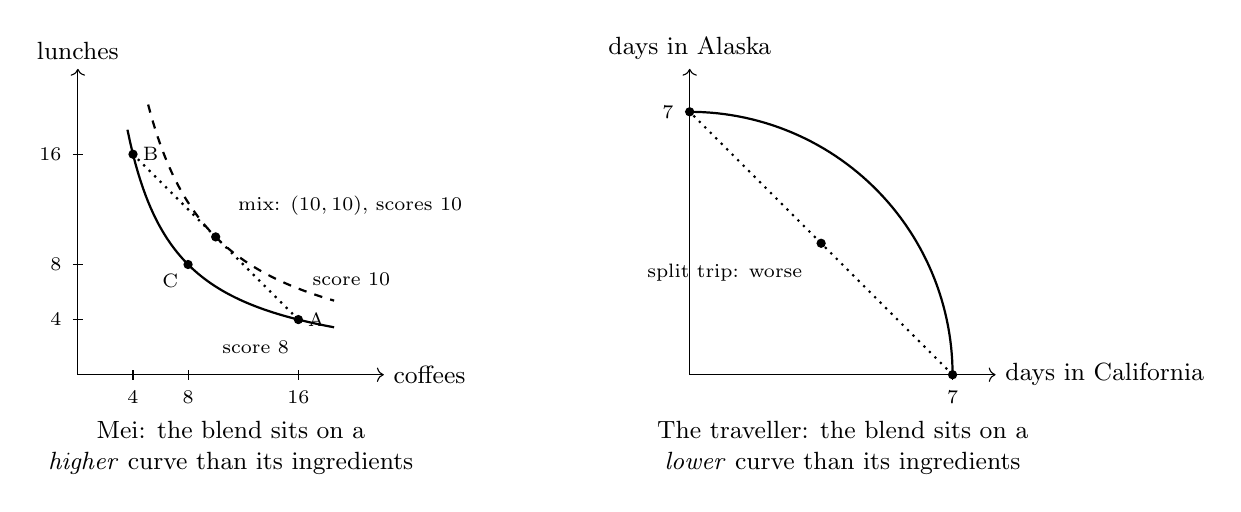
\begin{tikzpicture}[scale=1.05]
\begin{scope}
  \draw[->] (0,0) -- (3.7,0) node[right,font=\small] {coffees};
  \draw[->] (0,0) -- (0,3.7) node[above,font=\small] {lunches};
  \draw[thick,domain=0.60:3.10,samples=80] plot (\x, {1.7778/\x});
  \draw[thick,dashed,domain=0.85:3.10,samples=80] plot (\x, {2.7778/\x});
  \draw[dotted,thick] (2.667,0.667) -- (0.667,2.667);
  \fill (2.667,0.667) circle (1.6pt) node[right,font=\scriptsize] {A};
  \fill (0.667,2.667) circle (1.6pt) node[right,font=\scriptsize] {B};
  \fill (1.333,1.333) circle (1.6pt) node[below left,font=\scriptsize] {C};
  \fill (1.667,1.667) circle (1.6pt);
  \node[font=\scriptsize,anchor=west] at (1.82,2.05) {mix: $(10,10)$, scores 10};
  \node[font=\scriptsize,anchor=north] at (2.15,0.52) {score 8};
  \node[font=\scriptsize,anchor=west] at (2.72,1.15) {score 10};
  \foreach \p/\l in {0.667/4, 1.333/8, 2.667/16} {
    \draw (\p,-0.06) -- (\p,0.06); \node[font=\scriptsize,anchor=north] at (\p,-0.08) {\l};
    \draw (-0.06,\p) -- (0.06,\p); \node[font=\scriptsize,anchor=east] at (-0.08,\p) {\l};
  }
  \node[font=\small,anchor=north,align=center] at (1.85,-0.45)
    {Mei: the blend sits on a\\ \emph{higher} curve than its ingredients};
\end{scope}
\begin{scope}[xshift=7.4cm]
  \draw[->] (0,0) -- (3.7,0) node[right,font=\small] {days in California};
  \draw[->] (0,0) -- (0,3.7) node[above,font=\small] {days in Alaska};
  \draw[thick,domain=0:90,samples=60,variable=\t] plot ({3.18*cos(\t)},{3.18*sin(\t)});
  \draw[dotted,thick] (3.18,0) -- (0,3.18);
  \fill (3.18,0) circle (1.6pt);
  \fill (0,3.18) circle (1.6pt);
  \fill (1.59,1.59) circle (1.6pt);
  \node[font=\scriptsize,anchor=north east] at (1.48,1.46) {split trip: worse};
  \draw (3.18,-0.06) -- (3.18,0.06); \node[font=\scriptsize,anchor=north] at (3.18,-0.08) {7};
  \draw (-0.06,3.18) -- (0.06,3.18); \node[font=\scriptsize,anchor=east] at (-0.08,3.18) {7};
  \node[font=\small,anchor=north,align=center] at (1.85,-0.45)
    {The traveller: the blend sits on a\\ \emph{lower} curve than its ingredients};
\end{scope}
\end{tikzpicture}
\end{center}

\fwd{L2} Liking blends makes the set of best affordable baskets convex \src{L2 p.5}. Strictly liking
them makes it a single basket \src{L2 p.3}. The gap between those two conclusions is exactly the gap
between Axiom 5 and Axiom 5$'$, and it is one character in the statement.

\fwd{L2} Monotonicity, in its strict form, is what forces her to spend her whole budget
\src{L2 p.5}. It does not force her to buy some of everything: someone who cares only about coffee
still buys zero lunches \src{RS3 Q3.6}.

\fwd{L3} Strict convexity is the hypothesis that makes her shopping list move smoothly as prices
move \src{L3 p.4}. Without it her list can jump.
\section{How many lunches is one more coffee worth?}
\label{sec:q5}

\subsection{The scene: the same person, three different answers}

Walk along Mei's indifference curve, the one where every basket scores 8, and at each stop ask her
what one more coffee is worth.

\begin{center}
\begin{tabular}{@{}lll@{}}
\toprule
\textbf{Where she is} & \textbf{One more coffee is worth} & \textbf{Put another way} \\
\midrule
A: 16 coffees, 4 lunches & a quarter of a lunch & she needs 4 coffees to give up 1 lunch \\
C: 8 coffees, 8 lunches & one lunch & an even trade \\
B: 4 coffees, 16 lunches & four lunches & one coffee is worth 4 lunches to her \\
\bottomrule
\end{tabular}
\end{center}

Nothing about Mei changed between those rows. Only what she is already holding changed. At A she is
swimming in coffee and an extra one barely registers; at B coffee is scarce and she would give up a
great deal for one.

\subsection{The claim in plain words}

This exchange rate, and not ``how much satisfaction one more coffee gives,'' is the real quantity.
Section \ref{sec:q3} showed why: the second changes when you relabel the score and the first does
not.

\subsection{Where the number comes from}

Stay on one indifference curve, so that lunches are a function of coffees. The defining equation
holds for \emph{every} coffee amount along the curve, not at isolated points, and that is what makes
differentiating it legitimate \src{L1 p.16}:
\[
u\big( x_1, x_2(x_1) \big) = u^0 \qquad \text{for all } x_1 .
\]
Differentiate by the chain rule and rearrange:
\[
\frac{\partial u}{\partial x_1} + \frac{\partial u}{\partial x_2} \cdot \frac{dx_2}{dx_1} = 0
\qquad \Longrightarrow \qquad
\left. \frac{dx_2}{dx_1} \right|_{u^0} = - \frac{\MU_1}{\MU_2} .
\]

\begin{defn}[Marginal rate of substitution]
\[
\MRS_{2,1} = \left| \left. \frac{dx_2}{dx_1} \right|_{u^0} \right| = \frac{\MU_1}{\MU_2} .
\qquad \src{L1 pp.16--17}
\]
\end{defn}

For Mei this works out to $x_2 / x_1$, which produces the three numbers in the table: $4/16 = 0.25$,
then $8/8 = 1$, then $16/4 = 4$.

\begin{center}
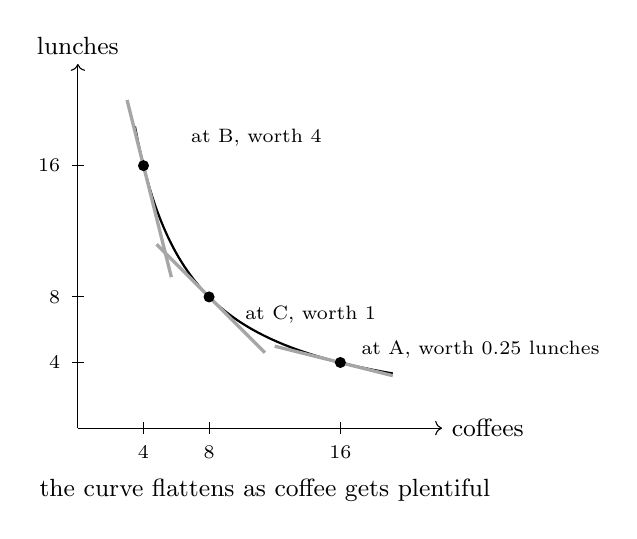
\begin{tikzpicture}[scale=1.25]
\draw[->] (0,0) -- (3.7,0) node[right,font=\small] {coffees};
\draw[->] (0,0) -- (0,3.7) node[above,font=\small] {lunches};
\draw[thick,domain=0.58:3.20,samples=90] plot (\x, {1.7778/\x});
\draw[very thick,gray!70] (2.00,0.833) -- (3.20,0.533);
\draw[very thick,gray!70] (0.80,1.867) -- (1.90,0.767);
\draw[very thick,gray!70] (0.50,3.334) -- (0.95,1.534);
\fill (2.667,0.667) circle (1.6pt);
\fill (1.333,1.333) circle (1.6pt);
\fill (0.667,2.667) circle (1.6pt);
\node[font=\scriptsize,anchor=west] at (2.78,0.80) {at A, worth $0.25$ lunches};
\node[font=\scriptsize,anchor=west] at (1.60,1.15) {at C, worth $1$};
\node[font=\scriptsize,anchor=west] at (1.05,2.95) {at B, worth $4$};
\foreach \p/\l in {0.667/4, 1.333/8, 2.667/16} {
  \draw (\p,-0.06) -- (\p,0.06); \node[font=\scriptsize,anchor=north] at (\p,-0.08) {\l};
  \draw (-0.06,\p) -- (0.06,\p); \node[font=\scriptsize,anchor=east] at (-0.08,\p) {\l};
}
\node[font=\small,anchor=north] at (1.9,-0.42)
  {the curve flattens as coffee gets plentiful};
\end{tikzpicture}
\end{center}

\subsection{Why this number survives relabelling and marginal utility does not}

\begin{prop}[Invariance of the MRS] If $v = h \circ u$ with $h$ differentiable and $h' > 0$, then
$u$ and $v$ give the same MRS everywhere. \src{L1 p.18, Exercise}, \src{RS2 Prop.\ 3}
\end{prop}

\skipnote
\begin{leftbar}
\small
By the chain rule $\partial v / \partial x_k = h'(u) \cdot \partial u / \partial x_k$ for every $k$.
Forming the ratio, the common factor $h'(u)$ is a nonzero number at the point in question and
cancels:
\[
\frac{\partial v / \partial x_1}{\partial v / \partial x_2}
= \frac{h'(u)\,\partial u / \partial x_1}{h'(u)\,\partial u / \partial x_2}
= \frac{\partial u / \partial x_1}{\partial u / \partial x_2} .
\]
The hypothesis $h' > 0$ is slightly stronger than $h$ strictly increasing, because a strictly
increasing differentiable function can have zero derivative at isolated points, as $t^3$ does at
zero, and the cancellation is unavailable there. The lecture writes $h' > 0$ \src{L1 p.18}, which is
the safe version.
\end{leftbar}

\begin{snugshade}
\noindent\textbf{The subscripts run in opposite orders in the two sources.} The lecture's
$\MRS_{2,1}$ is $\MU_1/\MU_2$ \src{L1 p.16}. J\&R defines $\MRS_{ij} = (\partial u/\partial x_i) /
(\partial u/\partial x_j)$, so J\&R's $\MRS_{12}$ is the same quantity \src{J\&R p.18}. Same number,
reversed indices. In any answer where the grader might use the other convention, write out the ratio
of marginal utilities explicitly.
\end{snugshade}

\subsection{Diminishing MRS is liking blends, seen from the side}

Mei's three numbers, $0.25$ then $1$ then $4$, fall as coffee becomes more plentiful. That is exactly
what it means to like blends, viewed one indifference curve at a time.

Maintain throughout: two goods, a differentiable score with both marginal utilities positive, so each
indifference curve is the graph of a decreasing function $x_2 = f(x_1)$.

\begin{prop}[Two goods, the lecture's Proposition 1.5] \label{prop:dmrs2}
She likes blends if and only if her MRS is weakly diminishing. \src{L1 p.18, ``Proof. Later.''}
\end{prop}

\skipnote
\begin{leftbar}
\small
Chain three equivalences.

First, liking blends is the same as every better-than set being convex, by the translation
proposition of \S\ref{sec:q4} and Theorem \ref{thm:qc}.

Second, under the maintained hypotheses the better-than set at level $u^0$ is
$\{ (x_1,x_2) : x_2 \ge f(x_1) \}$, the region on or above the curve. A set of that shape is convex
exactly when $f$ is a convex function, since the segment between two points of the curve lies in the
set precisely when
\[
t f(x_1^1) + (1-t) f(x_1^2) \ \ge \ f\big(t x_1^1 + (1-t)x_1^2\big).
\]

Third, a differentiable $f$ is convex exactly when $f'$ is nondecreasing, and
$\MRS_{2,1} = -f'$, so the MRS is nonincreasing exactly then.
\end{leftbar}

\begin{prop}[Any number of goods, the lecture's Proposition 1.4] \label{prop:dmrs}
If she likes blends, then every pairwise MRS is weakly diminishing. \src{L1 p.17}
\end{prop}

\skipnote
\begin{leftbar}
\small
Fix two goods and hold the others at some levels. The better-than sets of the restricted function are
the intersections of the original better-than sets with that two-dimensional slice, and an
intersection of convex sets is convex, so the restriction is quasi-concave by Theorem \ref{thm:qc}.
Proposition \ref{prop:dmrs2} applied to the restriction gives the conclusion.
\end{leftbar}

\subsection{What breaks: three goods}

The lecture says the result runs both ways for two goods \src{L1 p.17}, and that restriction is real.
With three goods a person can have a diminishing MRS between every pair and still dislike blends.

Take $u(x) = x_1 + (x_2 x_3)^{2/3}$ \src{RS2 Ex.\ 1.3}. The baskets $(16,0,0)$ and $(0,8,8)$ both
score 16. Blend them seven-eighths to one-eighth and you get $(14,1,1)$, which scores $14 + 1 = 15$.
Worse than both ingredients.

The reason is visible in the proof of Proposition \ref{prop:dmrs}. A pairwise MRS condition only ever
inspects a two-dimensional slice, and the blend that breaks things here moves in all three
coordinates at once. No slice sees it.

\fwd{L2} At an interior solution the first-order conditions divide into
$\MRS_{j,i} = p_i / p_j$ \src{L2 p.9}: her private exchange rate is driven to equal the market's. If
she privately values two coffees as one lunch while the shop trades them one for one, she sells
lunches and buys coffees until the rates meet. Diminishing MRS is what makes that meeting point a
maximum and not a minimum, which is why \S\ref{sec:q4} and this section are prerequisites for
Lecture 2 and not decoration.

\section{Four people at the same counter}
\label{sec:q6}

\subsection{The scene}

Four customers are each handed the same basket: 16 coffees and 4 lunches. They are equally keen on
coffee and lunch in the abstract, and they still value the basket completely differently, because
they differ in one thing only: how willing they are to substitute one for the other.

\begin{center}
\begin{tabular}{@{}llc@{}}
\toprule
\textbf{Customer} & \textbf{How she sees it} & \textbf{Value of the basket} \\
\midrule
Raj & a coffee and a lunch are interchangeable; he just counts items & 10 \\
Mei & she wants a decent amount of both & 8 \\
Ana & she only drinks coffee \emph{with} a lunch, one to one & 4 \\
Tom & he wants to go all in on one thing; mixtures annoy him & 16 \\
\bottomrule
\end{tabular}
\end{center}

Raj averages the two numbers. Ana is held hostage by whichever is scarcer, so the 12 extra coffees
are worth nothing to her. Mei is in between. Tom simply takes the larger number and ignores the
other, which as we will see puts him outside the theory.

\subsection{The four formulas}

\begin{align}
\text{Cobb-Douglas (Mei):} \quad & u(x) = \textstyle\prod_i x_i^{\alpha_i},
  && \alpha_i > 0, \ \textstyle\sum \alpha_i = 1, \\
\text{Linear (Raj):} \quad & u(x) = \textstyle\sum_i \alpha_i x_i, && \alpha_i > 0, \\
\text{Leontief (Ana):} \quad & u(x) = \min\{x_1, \dots, x_n\}, && \\
\text{CES:} \quad & u(x) = \Big( \textstyle\sum_i \alpha_i x_i^{\rho} \Big)^{1/\rho},
  && \alpha_i > 0, \ \textstyle\sum \alpha_i = 1, \ \rho < 1 .
\end{align}
\src{L1 pp.18--19}

\begin{center}
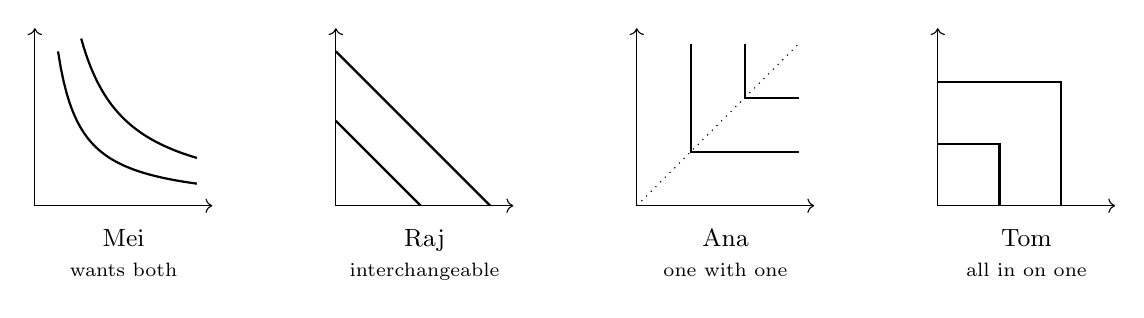
\begin{tikzpicture}[scale=0.98]
\begin{scope}
  \draw[->] (0,0) -- (2.3,0); \draw[->] (0,0) -- (0,2.3);
  \draw[thick,domain=0.30:2.1,samples=50] plot (\x,{0.6/\x});
  \draw[thick,domain=0.60:2.1,samples=50] plot (\x,{1.3/\x});
  \node[font=\small,anchor=north,align=center] at (1.15,-0.18) {Mei\\{\scriptsize wants both}};
\end{scope}
\begin{scope}[xshift=3.9cm]
  \draw[->] (0,0) -- (2.3,0); \draw[->] (0,0) -- (0,2.3);
  \draw[thick] (0,1.1) -- (1.1,0);
  \draw[thick] (0,2.0) -- (2.0,0);
  \node[font=\small,anchor=north,align=center] at (1.15,-0.18) {Raj\\{\scriptsize interchangeable}};
\end{scope}
\begin{scope}[xshift=7.8cm]
  \draw[->] (0,0) -- (2.3,0); \draw[->] (0,0) -- (0,2.3);
  \draw[dotted] (0,0) -- (2.1,2.1);
  \draw[thick] (0.7,2.1) -- (0.7,0.7) -- (2.1,0.7);
  \draw[thick] (1.4,2.1) -- (1.4,1.4) -- (2.1,1.4);
  \node[font=\small,anchor=north,align=center] at (1.15,-0.18) {Ana\\{\scriptsize one with one}};
\end{scope}
\begin{scope}[xshift=11.7cm]
  \draw[->] (0,0) -- (2.3,0); \draw[->] (0,0) -- (0,2.3);
  \draw[thick] (0,0.8) -- (0.8,0.8) -- (0.8,0);
  \draw[thick] (0,1.6) -- (1.6,1.6) -- (1.6,0);
  \node[font=\small,anchor=north,align=center] at (1.15,-0.18) {Tom\\{\scriptsize all in on one}};
\end{scope}
\end{tikzpicture}
\end{center}

Read the pictures against the table. Mei's curves bow toward the origin, which is liking blends. Raj's
are straight, so he likes blends but never strictly. Ana's have a corner on the diagonal, and the
flat arms are where extra coffee does nothing. Tom's bow the wrong way, and the region he prefers is
not convex.

\subsection{They are one family}

The three well-behaved customers are the same formula at three settings of one dial. Watch the value
of the 16-and-4 basket as $\rho$ falls, with equal weights:

\begin{center}
\begin{tabular}{@{}lcccccl@{}}
\toprule
$\rho$ & $1$ & $0.5$ & $0$ & $-1$ & $-5$ & $\to -\infty$ \\
\midrule
Value of $(16,4)$ & $10$ & $9$ & $8$ & $6.4$ & $4.59$ & $4$ \\
& Raj & & Mei & & & Ana \\
\bottomrule
\end{tabular}
\end{center}

The dial controls how much the weak link matters. At the top the customer simply averages; at the
bottom the scarcer good dictates everything and the surplus coffee is wasted.

\begin{prop}[The three limits and the curvature] For $\rho < 1$ the CES score is strictly
quasi-concave. As $\rho \to 1$ it becomes Raj's, as $\rho \to 0$ it becomes Mei's, and as
$\rho \to -\infty$ it becomes Ana's. \src{L1 p.19, ``Proof. Exercise.''}
\end{prop}

\skipnote
\begin{leftbar}
\small
Work on $\mathbb{R}^n_{++}$ and write $g(x) = \sum_i \alpha_i x_i^{\rho}$.

\emph{Curvature, $0 < \rho < 1$.} Each $t \mapsto t^\rho$ has second derivative
$\rho(\rho-1)t^{\rho-2} < 0$, so $g$ is strictly concave and therefore strictly quasi-concave. Since
$1/\rho > 0$, the map $t \mapsto t^{1/\rho}$ is strictly increasing and Proposition \ref{prop:qcinv}
finishes it.

\emph{Curvature, $\rho < 0$.} Now $\rho(\rho-1) > 0$, so $g$ is strictly convex and $-g$ is strictly
concave, hence strictly quasi-concave. Write $u = \tilde h(-g)$ with $\tilde h(s) = (-s)^{1/\rho}$;
substituting $r = -s > 0$ gives $d\tilde h/ds = -(1/\rho) r^{1/\rho - 1} > 0$ because $1/\rho < 0$,
so $\tilde h$ is strictly increasing and Proposition \ref{prop:qcinv} applies again. The sign of
$\rho$ is the only place the argument branches.

\emph{Limit $\rho \to 1$.} Substitute directly: the expression is $\sum_i \alpha_i x_i$ at
$\rho = 1$, and both base and exponent are continuous there with the base positive.

\emph{Limit $\rho \to 0$.} Take logarithms to isolate the indeterminacy:
$\ln u = \ln\big(\sum_i \alpha_i x_i^\rho\big) / \rho$. As $\rho \to 0$ the numerator tends to
$\ln 1 = 0$ and so does the denominator, so L'H\^opital applies in $\rho$. Using
$\frac{d}{d\rho} x_i^\rho = x_i^\rho \ln x_i$,
\[
\lim_{\rho \to 0} \ln u
= \frac{\sum_i \alpha_i \ln x_i}{\sum_i \alpha_i} = \sum_i \alpha_i \ln x_i ,
\]
and exponentiating gives $\prod_i x_i^{\alpha_i}$ \src{RS2 Q2.2}.

\emph{Limit $\rho \to -\infty$.} Let $m = \min_i x_i$ and let $A$ be the total weight on the goods
achieving that minimum, so $A \in (0,1]$. Factor $m$ out:
\[
u(x) = m \Big( \sum_i \alpha_i (x_i/m)^{\rho} \Big)^{1/\rho} .
\]
Every ratio $x_i/m$ is at least one, with equality exactly on the minimizing goods. A base above one
raised to $\rho \to -\infty$ tends to zero, so the inner sum tends to $A$. The exponent $1/\rho$
tends to zero and the base converges to something strictly positive, so the bracket tends to
$A^0 = 1$ and $u \to m$.
\end{leftbar}

Notice what the proof used. The sign of $\rho$ decided whether the inner function was concave or
convex, and in the negative case a strictly decreasing outer relabelling flipped it back. Nothing
used $\sum_i \alpha_i = 1$, which is a labelling convention and therefore, by \S\ref{sec:q3}, could
not have mattered.

\subsection{What breaks: Tom}

Push the dial the other way, $\rho \to +\infty$, and the formula becomes
$\max\{x_1, \dots, x_n\}$, which the lecture notes is not quasi-concave \src{L1 p.19}. Tom values the
16-and-4 basket at 16, ignoring the lunches entirely.

The one-line failure: a basket of 7 and 0 is worth 7 to him, and so is 0 and 7, but the even blend of
3.5 and 3.5 is worth only 3.5. The blend is worse than both ingredients, which is precisely the
inequality defining quasi-concavity, failing.

That is the split holiday of \S\ref{sec:q4} written as a formula, and it is why $\rho < 1$ is part of
the definition of the CES family instead of an afterthought.

\section{Where this goes}

\subsection{Lecture 2 spends the assumptions}

Lecture 2 adds one new object, a budget, and then runs everything from this lecture on it. Each
question above turns into a property of what she buys.

\begin{center}
\begin{tabular}{@{}p{0.30\textwidth} p{0.62\textwidth}@{}}
\toprule
\textbf{From Lecture 1} & \textbf{What Lecture 2 does with it} \\
\midrule
Completeness, transitivity & makes ``the best affordable basket'' a meaningful phrase at all \\
Continuity, plus a bounded budget set & guarantees a best affordable basket exists \src{L2 p.2} \\
Ordinality of the score & forces the optimality condition to be written in the MRS \src{L2 p.9} \\
She likes blends & makes the set of best baskets convex \src{L2 p.5} \\
She \emph{strictly} likes blends & makes the best basket unique \src{L2 p.3} \\
More is better, strictly & makes her spend her whole budget \src{L2 p.5} \\
Diminishing MRS & makes the tangency point a maximum \\
\bottomrule
\end{tabular}
\end{center}

\textbf{What looks similar and is not.} The letter $B$ means the better-than set here and the budget
set from Lecture 2 onward, and both are convex under the standing assumptions, and they are different
objects. Also, the budget set is convex because prices are linear, which is a fact about the shop and
not about the customer; convexity of preferences is Axiom 5. Uniqueness of her purchase needs both,
for different reasons.

\subsection{Lecture 3 and after}

Lecture 3 studies how well off she ends up, and two results from this lecture reappear in a form that
catches people. Quasi-concavity of her score lives in the space of baskets and comes from Axiom 5.
Quasi-\emph{convexity} of her standard of living lives in the space of prices and incomes and comes
from arithmetic on the budget line; it holds whether or not she likes blends \src{L3 p.3}. The words
rhyme and the results are unrelated.

The ordinality lesson of \S\ref{sec:q3} also returns. Her standard of living is not an ordinal
object, and the demand recovered from it by Roy's identity is, by exactly the cancellation in the
table on page \pageref{sec:q3} \src{L3 p.6}.

\subsection{Reading list}

\begin{itemize}
\item Preferences, utility and the axioms in textbook form, J\&R \S1.2.
\item Consumer demand and the budget set, J\&R \S1.3.
\item Indirect utility and expenditure, J\&R \S1.4.
\item Income and substitution effects, J\&R \S1.5.
\end{itemize}

\end{document}
